The composer and recorder player Claire Farrell approached me, asking for my opinion on how to notate an extended technique that she had been developing. 
The technique involves the recorder player covering the window hole with their index finger or hand, which results in the recorder producing a whistle like effect. 
Air pressure determines the pitch, and the degree to which the window hole is covered determines the fundamental's presence or lack thereof, with full occlusion of the window producing solely the harmonic. 

This is an ideal place in which to explore the ways in which we map actions into notation; the question becomes one of how this can be achieved in the most recognisable and orderly manner. 
Our goal of establishing a defined notation system is to ensure that it is as clear and easy to understand as possible. 

Thus began an informative exploration through the various ways that we can map sound onto an instrument. 
This is an especially interesting topic to me, as I am interested in the ways in which the semiotics of notation influence its parsing. 
We can treat this development of the notation of a new technique as a case study for best practices, and establish some ground rules on how the written form of Western art music can be adapted to accomodate new techniques that fall outside of the initial set.

\section{Literature Review}
Of particular interest is the work of Ellen Fallowfield, whose thesis, `CelloMap' website and recently, application, form a comprehensive and holistic review of the ways in which a performer may `map' actions onto a cello.\autocite[]{fallowfieldCelloMapHandbook2009,fallowfieldCelloMap}
This non-opinionated and genericized method of cataloguing actions sees its contents applicable where a more specific approach would fall short, ensuring that it does not fall out of date.
In a similar way, I aim to catalogue and genericize actions from a composer's perspective, providing a suite of tools with which a composer can construct a notation to suit any 

\subsection{Semiotics}
A brief overview of semiotics is necessary in order for any serious discussion to be had.
Semiotics, the study of signs (read: meaningful communication), was invented concurrently by Ferdinand de Saussure and Charles Sanders Peirce independent of one another.
The most appreciable difference between their models was that while Saussure held that signs were made up of a signifier (the form of the sign) and signified (its meaning), Pierce's model also had an interpretant; the object that the audience interprets the signified as (since it is impossible to replicate meaning perfectly).
Signifiers are then broken up into three discrete categories; 
\begin{itemize}
\item \emph{\gls{icon}}: which have a direct physical connection to the signified. Photographs are an example of icons.
\item \emph{\gls{index}}: which show evidence of the signified. The most common example being smoke indexing fire.
\item \emph{\gls{symbol}}: which have no resemblance between the signifier and the signified; their meaning must be culturally learned. Arabic numerals, the radioactive symbol, and flags are all symbols.
\end{itemize}

Finally, our signs have two channels of information.
\begin{itemize}
\item \emph{\gls{denotation}}: the basic or literal meaning of the sign (i.e.\ a picture of a rose signifies the flower of the genus \emph{Rosa} of the family \emph{Rosaceae})
\item \emph{\gls{connotation}}: the secondary, culturally inferred meaning; a rose might also signify passion or love, depending on the context.
\end{itemize}

Interpreting these signs is described as semiosis, which Tagg states is `simply the process by which meaning is produced and understood.'\autocite[156]{taggMusicMeaningsModern2013}
Semiosis happens constantly; the process of converting these words into the understanding of the concept of semiosis is, in itself, semiosis. 
This is an important step, though, as the interpretant which Peirce describes is unique to the audience; 
we construct meaning completely independently, informed by our past experiences and knowledge.\citetemp{citation needed - Pierce}
Thus, the same picture of an aunt's dog may be interpreted by the aunt as being a loving pet, whereas a neighbour might interpret the image as `the bloody dog that wakes me up at 6am'.

How does this relate to music, though? 
Floris Schuiling describes music notations as \begin{quotation}
`interfaces for imagining virtual musical relations'
\end{quotation}
which is an 
Looking at Western notation, we have several instances where a symbol may hold a different context depending on the interpreter's experience-- 
the same notation is used for a harmonic and a note that is meant to be played open on a French horn.\autocite[]{schuilingNotationCulturesEthnomusicology2019}
If a musician was given a piece of sheet music without any indicator of the instrument that it was written for, their experience (or lack thereof) with one of the instruments may influence how they choose to interpret the symbol.

Semiotics has seen a resurgence of interest with web design, where intuitive `notation' is sought after to reduce the `friction', or difficulty a user has navigating a site.
We can learn many things from the research that has been done into how to use skeuomorphic design to convey an element's function.
Our goal with constructing intuitive music notation is to reduce the `friction' just like a web designer.
We can use the connotations of existing symbols to help infer how we can construct new symbols.
As an example, the line that makes up a glissandi can be either straight, or wavy.
% , as seen in \autoref{fig:Glissando}.
% \begin{figure}
% 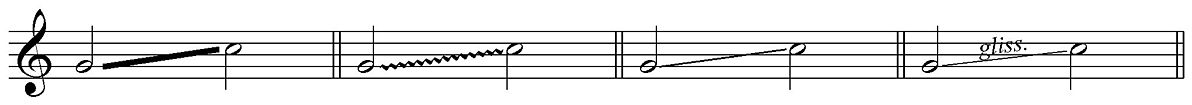
\includegraphics[width=10cm]{./resources/glissando.jpg}
% \caption{Various styles of glissandi}\label{fig:Glissando}
% \end{figure}
The similarity of the last two examples on the right to the notation for \emph{portamento} results in a connotation with those two types being continuous, rather than having discrete pitches.
Additionally, the interpretant's instrument may also influence the meaning to them- timpanists and trombonists are more likely to interpret glissandi as continuous changes, while pianists interpret step-wise due to the nature of their instruments.\autocite[]{}

Lastly, we need to understand that some symbols are not compatible with one another; a properly engraved work will never have an upbow and downbow on the same note, as the two symbols fulfill the same function.
This is what is known as a paradigmatic relationship; by virtue of the presence of one, it excludes the possibility of the other.
Other examples of paradigms would be the degree at which a French horn opens or mutes their instrument.
Looking at web design, we can draw a somewhat rough parallel to drop-down menus; there's only one slot that can be filled.

